% Clean bipartite redraw of plots/mismatch/2_1/wBMG_2_1.gml
% This is the weak best match graph of hybrid_network_2_1.gml (task_1d.py, step 2).
% Since wBMG edges only ever connect leaves of DIFFERENT species colours, the
% graph is naturally bipartite -- drawn here as two columns instead of a
% force-directed hairball.
% Compile with: pdflatex wBMG_2_1_clean.tex
\documentclass{article}
\usepackage[margin=1cm]{geometry}
\usepackage{tikz}
\usetikzlibrary{arrows.meta}

% matplotlib tab:blue / tab:orange, matching the gene_color values in the GML
\definecolor{tabblue}{rgb}{0.12156863,0.46666667,0.70588235}
\definecolor{taborange}{rgb}{1.0,0.49803922,0.05490196}

\begin{document}
\thispagestyle{empty}
\begin{center}
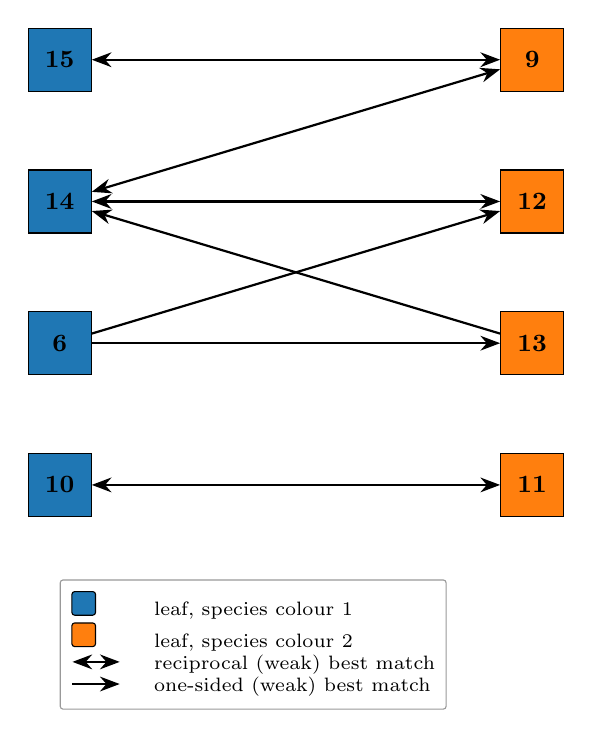
\begin{tikzpicture}[
  >={Stealth[length=2.5mm]},
  every node/.style={font=\small\bfseries},
  leafblue/.style={rectangle, fill=tabblue, text=black, minimum size=8mm, draw=black},
  leaforange/.style={rectangle, fill=taborange, text=black, minimum size=8mm, draw=black},
  mutual/.style={<->, thick},
  oneway/.style={->, thick},
]

% ---- left column: species colour 1 (blue) leaves ----
\node[leafblue] (l15) at (0, 0)    {15};
\node[leafblue] (l14) at (0, -1.8) {14};
\node[leafblue] (l6)  at (0, -3.6) {6};
\node[leafblue] (l10) at (0, -5.4) {10};

% ---- right column: species colour 2 (orange) leaves ----
\node[leaforange] (l9)  at (6, 0)    {9};
\node[leaforange] (l12) at (6, -1.8) {12};
\node[leaforange] (l13) at (6, -3.6) {13};
\node[leaforange] (l11) at (6, -5.4) {11};

% ---- edges (exactly as in wBMG_2_1.gml) ----
\draw[mutual] (l15) -- (l9);   % 15 <-> 9
\draw[mutual] (l14) -- (l9);   % 14 <-> 9
\draw[mutual] (l14) -- (l12);  % 14 <-> 12
\draw[oneway] (l13) -- (l14);  % 13 -> 14
\draw[mutual] (l10) -- (l11);  % 10 <-> 11
\draw[oneway] (l6)  -- (l12);  % 6 -> 12
\draw[oneway] (l6)  -- (l13);  % 6 -> 13

% ---- legend ----
\node[anchor=north west, font=\scriptsize, align=left, draw=black!40, fill=white, inner sep=4pt, rounded corners=1pt]
  at (0.0, -6.6) {%
  \begin{tabular}{@{}ll@{}}
    \tikz\node[leafblue, minimum size=3mm]{};   & leaf, species colour 1 \\
    \tikz\node[leaforange, minimum size=3mm]{}; & leaf, species colour 2 \\
    \tikz\draw[mutual] (0,0) -- (0.6,0);         & reciprocal (weak) best match \\
    \tikz\draw[oneway] (0,0) -- (0.6,0);         & one-sided (weak) best match \\
  \end{tabular}%
};

\end{tikzpicture}
\end{center}
\end{document}
